\documentclass[border=8pt]{standalone}
\usepackage{fontspec}
\setmainfont{TeX Gyre Heros}[Ligatures=TeXOff]
\XeTeXgenerateactualtext=1
\setsansfont{TeX Gyre Heros}
\usepackage{tikz}
\usetikzlibrary{arrows.meta,positioning,shapes.geometric,shapes.misc,shapes.symbols,fit,backgrounds,calc,chains}
\definecolor{ink}{HTML}{111827}
\definecolor{band}{HTML}{F3F4F6}
\definecolor{band2}{HTML}{E5E7EB}
\definecolor{accent}{HTML}{1D4ED8}
\definecolor{accentlight}{HTML}{DBEAFE}
\definecolor{warn}{HTML}{B91C1C}
\definecolor{warnlight}{HTML}{FEE2E2}
\definecolor{ok}{HTML}{047857}
\definecolor{oklight}{HTML}{D1FAE5}
\tikzset{
  >={Stealth[length=2.6mm]},
  box/.style={draw=ink, line width=0.6pt, rounded corners=9pt, fill=white, align=center,
              inner sep=4pt, font=\small},
  pill/.style={box, rounded corners=13pt},
  key/.style={box, fill=accentlight, draw=accent, line width=0.9pt},
  soft/.style={box, fill=band},
  dec/.style={draw=ink, line width=0.6pt, diamond, aspect=2.2, align=center, inner sep=1.5pt,
              font=\footnotesize, fill=white},
  arr/.style={->, draw=ink, line width=0.6pt},
  darr/.style={->, draw=ink, line width=0.6pt, dashed},
  lbl/.style={font=\footnotesize, fill=white, inner sep=1.5pt},
  layer/.style={draw=band2, fill=band, rounded corners=6pt},
  title/.style={font=\bfseries\small, align=left, anchor=west},
}
\begin{document}
\sffamily\hyphenpenalty=10000\exhyphenpenalty=10000

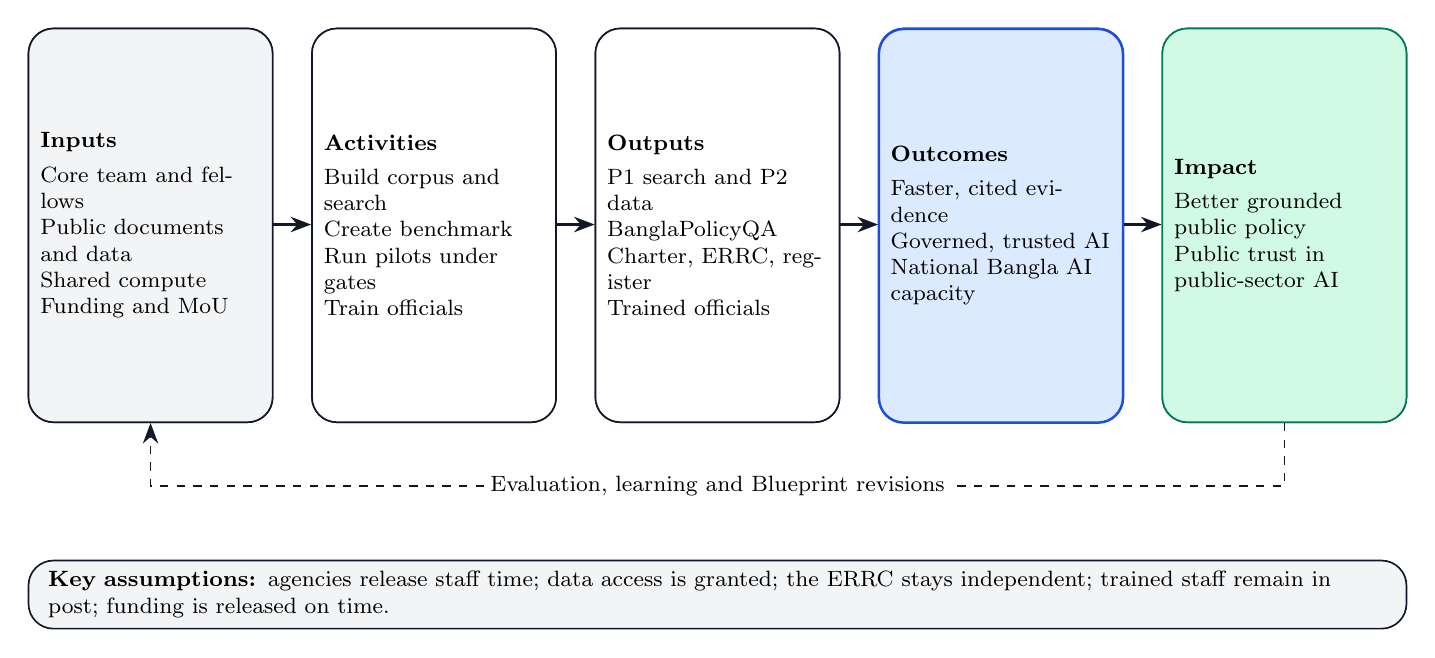
\begin{tikzpicture}
\tikzset{tc/.style={box, minimum width=31mm, minimum height=50mm, text width=28mm, font=\footnotesize, align=left, anchor=north}}
\foreach \i/\x in {1/0,2/36,3/72,4/108,5/144} \node[tc] (t\i) at (\x mm,0) {};
\node[tc, fill=band] at (t1.north) {\textbf{Inputs}\\[1mm]Core team and fellows\\Public documents and data\\Shared compute\\Funding and MoU};
\node[tc] at (t2.north) {\textbf{Activities}\\[1mm]Build corpus and search\\Create benchmark\\Run pilots under gates\\Train officials};
\node[tc] at (t3.north) {\textbf{Outputs}\\[1mm]P1 search and P2 data\\BanglaPolicyQA\\Charter, ERRC, register\\Trained officials};
\node[tc, fill=accentlight, draw=accent, line width=0.9pt] at (t4.north) {\textbf{Outcomes}\\[1mm]Faster, cited evidence\\Governed, trusted AI\\National Bangla AI capacity};
\node[tc, fill=oklight, draw=ok] at (t5.north) {\textbf{Impact}\\[1mm]Better grounded public policy\\Public trust in public-sector AI};
\foreach \i/\j in {1/2,2/3,3/4,4/5} \draw[arr, line width=1pt] (t\i.east |- 0,-25mm) -- (t\j.west |- 0,-25mm);
\node[soft, minimum width=175mm, text width=170mm, font=\footnotesize, align=left] (as) at (72mm,-72mm) {\textbf{Key assumptions:} agencies release staff time; data access is granted; the ERRC stays independent; trained staff remain in post; funding is released on time.};
\draw[darr] (t5.south) -- ++(0,-8mm) -| node[lbl, pos=0.25]{Evaluation, learning and Blueprint revisions} (t1.south);
\end{tikzpicture}
\end{document}
